% Chapter Chapter 3 For Reproducible Research in R and RStudio
% Christopher Gandrud
% Created: 16/07/2012 05:45:03 pm CEST
% Updated: 3 September 2012




\chapter{Getting Started with R, RStudio, and knitr}\label{GettingStarted}

If you have rarely or never used R before the first two sections of this chapter give you enough information to be able to get started and understand the code I use in this book. For more detailed introductions to R please refer to the related resources I mentioned in chapter \ref{WhatNot}. Experienced R users might want to skip the first two sections of the chapter. This chapter also gives a brief overview of RStudio. It highlights the key features of main RStudio panel (what appears when you open RStudio) and some of its key features for reproducible research. Finally, I discuss the basics of the {\emph{knitr}} package and how it is integrated into RStudio.

%%%%%%%%%%%%% Using R
\section{Using R: the basics}

As a computer language, R has FILL in

This section covers some of the very basic syntax in R to get you started. If you have little experience with R, reading this section will make it much easier for you to follow along with the examples in the book. I cover the key components of the R language including:

\begin{itemize}
    \item objects \& assignment,
    \item component selection,
    \item functions, commands, and arguments,
    \item libraries.
\end{itemize}

Before discussing each of these components let's open up R and look around.\footnote{Please see Chapter \ref{Intro} for instructions on how to install R.} When you open up R you should get a window that looks something like what you see in Figure \ref{RBlankMain}.\footnote{This figure and almost all screenshots in this book are from a computer using the Mac OS 10.8 operating system.} This window is the {\bf{R console}}\index{R console}. Under the session\index{session information} information--what version of R you are using, your workspace, and so on--you should see a {\tt{\textgreater}}. This is where you enter R code.\footnote{If you are using a Unix-like system such as Ubuntu or Mac OS 10, you can an application called the Terminal\index{Terminal}. If you have installed R on your computer you can type {\tt{r}} into the terminal and then the {\tt{Enter}} or {\tt{Return}} key it will begin a new R session. You know if a new R session has started if you get the same startup information is printed in the Terminal window.} To run R code that you have typed into the console type the {\tt{Enter}} or {\tt{Return}} key. Now that we have a new R session open we can get started. 

\begin{figure}[th!]
    \caption{R Startup Console}
    \label{RBlankMain}
    \begin{center}
    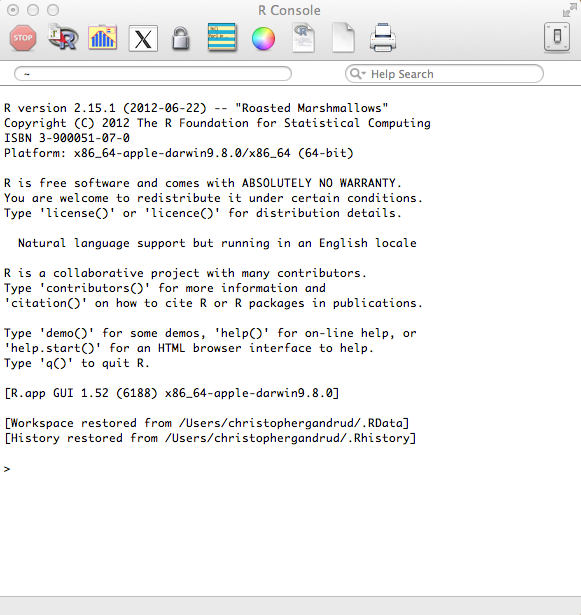
\includegraphics[scale=0.4]{/git_repositories/Rep-Res-Book/Source/Children/Chapter3/images3/BlankRConsole.png}
    \end{center}
\end{figure}

\subsection{Objects}

You will probably have read that `R is an object-oriented\index{object-oriented} language'.  What are objects? Objects are like the R language's nouns. They are things, such as a list of numbers, a data set, a word, a table of results from some analysis, and so on. Saying that R is `object-oriented' just means that R is focused on doing actions to objects. We will talk about the actions--commands and functions--later in this section. For now let's create a few objects.

\paragraph{Numeric \& string objects}

Different types of objects have different classes\index{object classes}. Let's make two basic objects of the numeric and character classes. We can choose almost any name we want for our objects.\footnote{Objects must begin with an alphabetic character and cannot have spaces.} Let's call our numeric object {\emph{Number}}. To put something into the object we use the {\bf{assignment operator}}: {\tt{\textless -}}. Let's assign the number 10 to our Number object.

\begin{knitrout}
\definecolor{shadecolor}{rgb}{0.969, 0.969, 0.969}\color{fgcolor}\begin{kframe}
\begin{alltt}
Number <- 10
\end{alltt}
\end{kframe}
\end{knitrout}


\noindent To see the contents of our object, just type its name.

\begin{knitrout}
\definecolor{shadecolor}{rgb}{0.969, 0.969, 0.969}\color{fgcolor}\begin{kframe}
\begin{alltt}
Number
\end{alltt}
\begin{verbatim}
## [1] 10
\end{verbatim}
\end{kframe}
\end{knitrout}


\noindent Lets's briefly breakdown this output. \texttt{10} is clearly the contents of {\emph{Number}}. The double hash (\texttt{\#\#}) is included in the output by {\emph{knitr}} to tell you that this is output rather than R code.\footnote{This makes it easier to copy and past code included in a presentation document by {\emph{knitr}}.} Finally, \texttt{[1]} is the row number of the object that 10 is on. Clearly our object only has one row.   

Creating a character object is very similar. The only difference is that we enclose the character string (letters in a word for example) inside of quotation marks ({\tt{""}}). To create an object called {\emph{Words}} that contains a character string ``Hello World".

\begin{knitrout}
\definecolor{shadecolor}{rgb}{0.969, 0.969, 0.969}\color{fgcolor}\begin{kframe}
\begin{alltt}
Words <- \hlstring{"Hello World"}
\end{alltt}
\end{kframe}
\end{knitrout}



An object's class is important to keep in mind as it determines what things we can do to it. For example you cannot take the mean of a character class object like the {\emph{Words}} object we created earlier:

\begin{knitrout}
\definecolor{shadecolor}{rgb}{0.969, 0.969, 0.969}\color{fgcolor}\begin{kframe}
\begin{alltt}
\hlfunctioncall{mean}(Words)
\end{alltt}


{\ttfamily\noindent\textcolor{warningcolor}{\#\# Warning: argument is not numeric or logical: returning NA}}\begin{verbatim}
## [1] NA
\end{verbatim}
\end{kframe}
\end{knitrout}


\noindent Trying to find the mean of our {\emph{Words}} object gave us a warning message and returned the value {\tt{NA}}\index{NA}: not applicable. You can also think of {\tt{NA}} to mean missing. To find out what class an object has use the {\tt{class}} command. For example:

\begin{knitrout}
\definecolor{shadecolor}{rgb}{0.969, 0.969, 0.969}\color{fgcolor}\begin{kframe}
\begin{alltt}
\hlfunctioncall{class}(Words)
\end{alltt}
\begin{verbatim}
## [1] "character"
\end{verbatim}
\end{kframe}
\end{knitrout}


\paragraph{Vector \& data frame Objects}

Sp far we have only looked at objects with a single number or string.\footnote{These might be called scalar objects, though in R scalars are just vectors with a length of 1.} Clearly we want to be using objects--data sets--that have many strings and numbers. In R these are usually {\bf{data frame}}\index{data frame} type objects and are roughly equivalent to the type of data structure you would be familiar with from using a program such as Microsoft Excel. We will be using data frames extensively throughout the book. It is also useful to cover other, simpler types of objects, primarily vectors. Vectors are R's ``workhorse".\cite{Matloff2011} Knowing how to use vectors\index{vector} will be especially helpful when we clean up raw data in Chapter \ref{DataClean} and make tables in Chapter \ref{TablesChapter}.\footnote{If you want information about other types of R objects such as lists\index{list} and matrices\index{matrix}, Chapter 1 of Norman Matloff's book\cite{Matlof2011} is a really good place to look.} \\[0.25cm]

\noindent {\bf{Vectors}}: \\[0.25cm] Vectors are the ``fundamental data type"\cite{Matloff2011} in R. They are simply an ordered group of numbers, character strings, and so on.\footnote{In a vector every member of the group must be of the same type. Lists are similar to vectors, but allow you to have different types.} It may be useful to think of basically all other data types as complicated forms of vectors. For example, data frames are basically multiple vectors of the same length--i.e. they have the same number of rows--attached together. 

Let's create a very simple numeric vector containing the numbers 1, 17, 24, and 6. To do this we will use the \texttt{c} (concatenate)\index{concatenate} function:

\begin{knitrout}
\definecolor{shadecolor}{rgb}{0.969, 0.969, 0.969}\color{fgcolor}\begin{kframe}
\begin{alltt}
NumericVect <- \hlfunctioncall{c}(2.8, 2, 14.8)

\hlcomment{# Show NumericVect's contents}
NumericVect
\end{alltt}
\begin{verbatim}
## [1]  2.8  2.0 14.8
\end{verbatim}
\end{kframe}
\end{knitrout}


Vectors of character strings are created in a similar way. The only major difference is that each character string is enclosed in quotation marks like this:

\begin{knitrout}
\definecolor{shadecolor}{rgb}{0.969, 0.969, 0.969}\color{fgcolor}\begin{kframe}
\begin{alltt}
CharacterVect <- \hlfunctioncall{c}(\hlstring{"Albania"}, \hlstring{"Botswana"}, \hlstring{"Cambodia"})

\hlcomment{# Show CharacterVect's contents}
CharacterVect
\end{alltt}
\begin{verbatim}
## [1] "Albania"  "Botswana" "Cambodia"
\end{verbatim}
\end{kframe}
\end{knitrout}


To give you a preview of what we are going to do when we start working with real data sets, lets combine the two vectors {\emph{NumericVect}} and {\emph{CharacterVect}} into a new object with the \texttt{cbind}\index{cbind} function. This function binds the two vectors together as if they were different columns.

















